% ===========================================================================
%  Actividad: Anonimización de datos — ¿En qué minuto se perdió la partida?
%  Héctor Manuel Morán Maldonado
%  Compilar:  python scripts/anonimizar.py  &&  latexmk -pdf reporte_anonimizacion.tex
% ===========================================================================
\documentclass[11pt,letterpaper]{article}

\usepackage[utf8]{inputenc}
\usepackage[T1]{fontenc}
\usepackage[spanish,es-tabla,es-nodecimaldot]{babel}
\usepackage{lmodern}
\usepackage{microtype}
\usepackage[margin=2.5cm,top=2.6cm,bottom=2.6cm]{geometry}
\usepackage{graphicx}
\usepackage{booktabs}
\usepackage{array}
\usepackage{float}
\usepackage{xcolor}
\usepackage{amsmath}
\usepackage{enumitem}
\usepackage{caption}
\usepackage{fancyhdr}
\usepackage{titlesec}
\usepackage[hidelinks]{hyperref}

\emergencystretch=2em
\definecolor{azul}{HTML}{2A78D6}
\definecolor{naranja}{HTML}{EB6834}
\definecolor{tinta}{HTML}{1A1A19}
\definecolor{suave}{HTML}{52514E}
\definecolor{papel}{HTML}{F4F6F8}

\captionsetup{font=small,labelfont={bf,color=azul},width=.92\linewidth}
\titleformat{\section}{\Large\bfseries\color{tinta}}{\thesection}{.7em}{}
\titleformat{\subsection}{\large\bfseries\color{suave}}{\thesubsection}{.7em}{}
\titlespacing*{\section}{0pt}{2.2ex plus 1ex minus .2ex}{1.2ex plus .2ex}

\pagestyle{fancy}\fancyhf{}
\renewcommand{\headrulewidth}{.4pt}
\fancyhead[L]{\footnotesize\color{suave}Anonimización de datos · ¿En qué minuto se perdió la partida?}
\fancyhead[R]{\footnotesize\color{suave}H. M. Morán Maldonado}
\fancyfoot[C]{\footnotesize\color{suave}\thepage}

\newsavebox{\cajaresp}
\newenvironment{respuesta}[1]
  {\par\medskip\setlength{\fboxsep}{10pt}%
   \begin{lrbox}{\cajaresp}%
   \begin{minipage}{\dimexpr\linewidth-2\fboxsep-3pt\relax}%
   \color{tinta}\textcolor{azul}{\textbf{#1}}\par\smallskip\ignorespaces}
  {\end{minipage}%
   \end{lrbox}%
   \noindent\textcolor{azul}{\rule[-\dp\cajaresp]{3pt}{\dimexpr\ht\cajaresp+\dp\cajaresp\relax}}%
   \colorbox{papel}{\usebox{\cajaresp}}\par\medskip}

\newcommand{\dato}[1]{\textbf{\textcolor{azul}{#1}}}
\newcommand{\nPartidas}{7}
\newcommand{\nPartidasCinco}{6}
\newcommand{\nParticipantes}{68}
\newcommand{\nCuadros}{2\,054}
\newcommand{\nEventos}{6\,877}
\newcommand{\nFugas}{0}
\newcommand{\nPuuid}{68}
\newcommand{\nRiotId}{81}
\newcommand{\nCampos}{19}
\newcommand{\nSuprimidos}{10}
\newcommand{\nSeudo}{2}
\newcommand{\nGeneral}{3}
\newcommand{\pctUnicosCrudo}{100{,}0}
\newcommand{\pctUnicosGen}{100{,}0}
\newcommand{\pctUnicosSinCampeon}{63{,}3}
\newcommand{\pctUnicosCampeon}{75{,}0}
\newcommand{\kMinSinCampeon}{1}
\newcommand{\compUnicas}{6}
\newcommand{\compTotal}{6}


\begin{document}

% ===========================================================================
\begin{titlepage}
\thispagestyle{empty}
\centering
\vspace*{0.6cm}

\includegraphics[width=6.4cm]{assets/logo-up.png}

\vspace{1.1cm}
{\large\color{suave}Especialidad en Ciencia de Datos\par}
\vspace{0.25cm}
{\large\color{suave}Visualización de datos y narración de historias\par}

\vspace{1.5cm}
{\color{azul}\rule{\linewidth}{1.6pt}}
\vspace{0.85cm}

{\Huge\bfseries Anonimización de datos\par}
\vspace{0.45cm}
{\LARGE Aplicada al corpus del proyecto\\[.25cm]
 \emph{¿En qué minuto se perdió la partida?}\par}
\vspace{0.35cm}
{\large\color{suave} Partidas de League of Legends · API de Riot Games\par}

\vspace{0.85cm}
{\color{azul}\rule{\linewidth}{1.6pt}}

\vfill

\begin{minipage}{0.46\linewidth}
  \raggedright
  {\color{suave}\small ALUMNO}\par\smallskip
  {\large Héctor Manuel Morán Maldonado\par}
\end{minipage}\hfill
\begin{minipage}{0.46\linewidth}
  \raggedleft
  {\color{suave}\small PROFESOR}\par\smallskip
  {\large Dr.\ Rodolfo Rubén Álvarez González\par}
\end{minipage}

\vspace{1.1cm}
{\color{suave}\rule{\linewidth}{.4pt}}
\vspace{0.45cm}

{\color{suave}\small
\nPartidas{} partidas · \nParticipantes{} participantes · \nCuadros{} cuadros-jugador · \nEventos{} eventos\\
Todas las cifras las genera \texttt{scripts/anonimizar.py} a partir de los JSON crudos\par}
\end{titlepage}

\tableofcontents
\newpage

% ===========================================================================
\section{Introducción: la naturaleza de la base de datos}

El proyecto \emph{¿En qué minuto se perdió la partida?} reconstruye partidas de
League of Legends minuto a minuto para identificar cuándo cambia su dirección. Los
datos vienen del endpoint \texttt{match-v5} de la API oficial de Riot Games, que por
cada partida entrega dos documentos JSON: el \emph{registro} (resultado, campeones,
roles, estadísticas finales) y la \emph{línea temporal} (el estado de los diez
jugadores cuadro por cuadro, más cada evento con su marca de tiempo).

\begin{respuesta}{Qué tipo de información es}
No es información crediticia ni de salud: es \textbf{registro de comportamiento
dentro de un juego}. Pero sí contiene \textbf{datos personales}, porque cada partida
identifica a sus diez jugadores por su cuenta. Y nueve de esos diez son terceros que
no forman parte del proyecto ni consintieron estar en él. La política para
desarrolladores de Riot prohíbe además desanonimizar a los jugadores.
\end{respuesta}

\noindent Para esta actividad se usa el corpus piloto del proyecto: \dato{\nPartidas{}
partidas públicas} de ejemplo del repositorio de esquemas de la API
(\texttt{MingweiSamuel/riotapi-schema}). Son partidas reales, de otras personas, y por
eso mismo son un buen banco de prueba: el proceso que se describe aquí es el que
correrá sin cambios sobre las partidas propias cuando se descarguen. De los JSON se
derivan cuatro tablas:

\begin{table}[H]\centering\small
\caption{Las cuatro tablas del proyecto, ya anonimizadas.}
\begin{tabular}{llrl}
\toprule
Tabla & Una fila es & Filas & Llave \\
\midrule
\texttt{partidas} & una partida & \nPartidas & \texttt{partida} (seudónimo) \\
\texttt{participantes} & un jugador en una partida & \nParticipantes & \texttt{partida}, \texttt{participantId} \\
\texttt{cuadros} & un jugador en un minuto & \nCuadros & \texttt{partida}, \texttt{minuto}, \texttt{participantId} \\
\texttt{eventos} & un suceso con marca de tiempo & \nEventos & \texttt{partida}, \texttt{ms} \\
\bottomrule
\end{tabular}
\end{table}

% ===========================================================================
\section{Identificación de variables: qué se anonimiza y qué no}

Siguiendo la clasificación vista en clase, cada campo del JSON cae en uno de cuatro
tipos de atributo. La clasificación se hizo \textbf{midiendo}, no leyendo la
documentación: se buscó cada valor de identificador en todas las rutas del JSON para
saber dónde aparece realmente.

\sloppy
\begin{itemize}[leftmargin=1.4em,itemsep=.35em]
  \item \textbf{Identificadores directos.} \texttt{puuid}, \texttt{summonerId},
        \texttt{summonerName}, \texttt{riotIdGameName} y \texttt{riotIdTagline}
        (juntos forman el Riot ID, \emph{nombre\#etiqueta}, que es como un jugador
        aparece en el juego), y \texttt{profileIcon}. El \texttt{puuid} aparece en
        \textbf{tres} lugares: en cada participante, en la lista
        \texttt{participants} de los metadatos del registro, y en la lista
        \texttt{participants} de la línea temporal.
  \item \textbf{Cuasi-identificadores.} Solos no nombran a nadie; combinados, sí.
        \begin{itemize}[itemsep=.15em]
          \item \texttt{matchId} y \texttt{gameId}: el caso más grave. Con
                \texttt{matchId}, cualquiera con una llave de la API pide la
                partida y recibe de vuelta los diez Riot ID. Es un identificador
                de \emph{diez} personas a la vez.
          \item \texttt{gameCreation} y los demás \emph{timestamps} absolutos:
                fecha y hora exactas, que además revelan los hábitos de juego.
          \item \texttt{summonerLevel}: el nivel de cuenta separa jugadores casi
                tanto como un nombre.
          \item \texttt{championName} con \texttt{teamPosition}, y sobre todo la
                \textbf{composición} de los diez campeones de una partida.
        \end{itemize}
  \item \textbf{Datos sensibles.} En el sentido de la clase (salud, salario,
        creencias) \textbf{no hay}. Lo más cercano es la hora a la que alguien
        juega, que es un patrón de conducta; por eso la fecha se generaliza.
  \item \textbf{Datos no sensibles.} Oro, experiencia, KDA, daño, visión, objetivos,
        posiciones en el mapa y los \emph{timestamps} de cuadros y eventos, que son
        relativos al inicio de la partida. Son el objeto de estudio y se conservan.
\end{itemize}
\fussy

\noindent La tabla~\ref{tab:politica} es la política completa. No es una copia
escrita a mano: la genera el mismo script que aplica la anonimización, así que no
puede desincronizarse del código.

\begin{table}[H]
\centering
\small
\caption{Política de anonimización, campo por campo (generada desde el script).}
\label{tab:politica}
\begin{tabular}{p{4.2cm}p{2.3cm}p{4.6cm}p{2.4cm}}
\toprule
Campo & Nivel & Técnica & Columna de salida \\
\midrule
riotIdGameName / riotIdName & participante & Supresión & — \\
riotIdTagline & participante & Supresión & — \\
summonerName & participante & Supresión & — \\
summonerId & participante & Supresión & — \\
profileIcon & participante & Supresión & — \\
puuid & participante & Seudonimización (HMAC-SHA256) & jugador, es\_propio, cuenta \\
metadata.participants & partida & Supresión & — \\
matchId & partida & Seudonimización (HMAC-SHA256) & partida \\
gameId & partida y eventos & Supresión & — \\
gameName, tournamentCode & partida & Supresión & — \\
gameCreation & partida & Generalización (fecha → mes) & mes \\
gameStartTimestamp, gameEndTimestamp & partida & Supresión & — \\
gameVersion & partida & Generalización (versión → parche) & parche \\
summonerLevel & participante & Generalización (bandas) & bandaNivel \\
victimDamage*[].name & eventos & Supresión (no se exporta) & — \\
championName, teamPosition & participante & Se conserva (análisis) & campeon, rol \\
timestamp de cuadros y eventos & cuadros, eventos & Se conserva (relativo al inicio) & ms, minuto \\
position \{x, y\} & cuadros, eventos & Se conserva & x, y \\
oro, xp, KDA, daño, visión, objetivos & todos & Se conserva (no identifica) & — \\
eventos de la tabla pública & eventos (público) & Minimización: solo torres y monstruos épicos; sin posición ni víctima & eventos\_equipo \\
\bottomrule
\end{tabular}
\end{table}


% ===========================================================================
\section{Técnicas de anonimización aplicadas}

\subsection{Supresión}
Los \dato{\nSuprimidos{} campos} marcados como «Supresión» simplemente no se
escriben. Es la técnica para todo lo que no aporta al análisis: el proyecto no
necesita saber cómo se llama nadie. También se suprimen campos anidados que no se
ven a primera vista, como \texttt{gameId} dentro de cada evento de la línea
temporal, y las listas \texttt{victimDamage*}, que no se exportan.

\subsection{Seudonimización con HMAC}
Dos identificadores no se pueden suprimir sin romper el análisis, porque son
\emph{llaves}: \texttt{matchId} une las cuatro tablas y \texttt{puuid} permite
distinguir al jugador propio de los demás. Se reemplazan por un seudónimo:
\[
  \texttt{partida} = \mathrm{HMAC\text{-}SHA256}(\text{llave},\ \texttt{matchId})\ \text{(12 caracteres)}
\]

\noindent ¿Por qué HMAC y no un hash simple? Porque un \texttt{matchId} tiene la
forma \texttt{EUW1\_} seguida de un número casi secuencial: se puede enumerar el
espacio, calcular \(\mathrm{sha256}\) de cada candidato y revertir el hash. Es
exactamente lo que pasó con los taxis de Nueva York de la presentación de clase: se
publicaron los números de licencia con un hash MD5 simple y se revirtieron todos en
minutos (Pandurangan, 2014). Con HMAC, sin la llave no hay nada que enumerar.

\begin{respuesta}{La llave es efímera, y eso cambia la técnica}
El script genera una llave aleatoria en cada corrida y \textbf{no la guarda}. Al
terminar, no existe ninguna tabla de correspondencia: ni el propio autor puede
regresar de un seudónimo a la persona. En ese caso deja de ser seudonimización
(que el RGPD sigue considerando dato personal, art.~4.5) y se vuelve anonimización
de esos campos. Si hace falta unir dos corridas, la llave se pasa por la variable
de entorno \texttt{LOL\_ANON\_KEY}, que vive fuera del repositorio.
\end{respuesta}

\noindent Consecuencia práctica: con llave efímera, después de seudonimizar ya no se
puede saber cuál de los diez jugadores soy yo. Por eso el script recibe el
\texttt{puuid} propio (\texttt{--mi-puuid}) y escribe la columna \texttt{es\_propio}
\emph{antes} de aplicar el HMAC. Es lo único que se decide con el identificador real.

\subsection{Generalización}
Tres campos se conservan con menos detalle:
\begin{itemize}[leftmargin=1.4em,itemsep=.25em]
  \item \textbf{Fecha → mes.} \texttt{gameCreation} (milisegundos exactos) pasa a
        \texttt{2026-03}. El análisis por parche no necesita el día.
  \item \textbf{Versión → parche.} \texttt{13.16.525.6443} pasa a \texttt{13.16}.
  \item \textbf{Nivel de cuenta → bandas:} 1--99, 100--299, 300--599 y 600+.
\end{itemize}

\subsection{Lo que se conserva, y por qué}
Campeón, rol, equipo, resultado y todas las estadísticas de juego se conservan:
son la materia prima de la pregunta del proyecto. Los \emph{timestamps} de la línea
temporal también, porque son relativos al inicio (el minuto 22 de una partida no
dice cuándo se jugó). Esa decisión tiene un costo, que se mide en la
sección~\ref{sec:riesgo}.

% ===========================================================================
\section{Ejemplo con datos ficticios}

Todos los valores de esta sección son inventados. Los seudónimos sí se calcularon
con la función real del script, usando una llave de demostración.

\begin{table}[H]\centering\small
\caption{Un participante antes y después. Valores ficticios.}
\begin{tabular}{p{4.2cm}p{5.6cm}p{5cm}}
\toprule
Campo & Antes (JSON crudo) & Después (CSV) \\
\midrule
\texttt{riotIdGameName\#Tagline} & \texttt{SombraDelNorte\#LAN1} & \textcolor{suave}{— suprimido —} \\
\texttt{summonerId} & \texttt{Qm2x8V-ficticio} & \textcolor{suave}{— suprimido —} \\
\texttt{profileIcon} & \texttt{5437} & \textcolor{suave}{— suprimido —} \\
\texttt{puuid} & \texttt{Xk3pQ9-ficticio-puuid-7HbL2w} & \texttt{jugador = baa18e16cee7} \\
\texttt{summonerLevel} & \texttt{347} & \texttt{bandaNivel = 300–599} \\
\texttt{championName} & \texttt{Ahri} & \texttt{campeon = Ahri} \\
\texttt{teamPosition} & \texttt{MIDDLE} & \texttt{rol = MIDDLE} \\
\texttt{kills / deaths / assists} & \texttt{7 / 3 / 9} & \texttt{7 / 3 / 9} \\
\texttt{goldEarned} & \texttt{12\,840} & \texttt{12\,840} \\
\bottomrule
\end{tabular}
\end{table}

\begin{table}[H]\centering\small
\caption{Una partida antes y después. Valores ficticios.}
\begin{tabular}{p{4.2cm}p{5.6cm}p{5cm}}
\toprule
Campo & Antes (JSON crudo) & Después (CSV) \\
\midrule
\texttt{matchId} & \texttt{LA1\_1488203317} & \texttt{partida = 24f61cd6497b} \\
\texttt{gameId} & \texttt{1488203317} & \textcolor{suave}{— suprimido —} \\
\texttt{gameCreation} & \texttt{1773528060000} (14-mar-2026, 22:41) & \texttt{mes = 2026-03} \\
\texttt{gameVersion} & \texttt{16.5.712.4321} & \texttt{parche = 16.5} \\
\texttt{queueId} & \texttt{420} & \texttt{cola = 420} \\
\texttt{gameDuration} & \texttt{1715} (segundos) & \texttt{duracionMin = 28.58} \\
\bottomrule
\end{tabular}
\end{table}

\noindent Lo que hay que notar es la fila de \texttt{matchId}. Una versión ingenua
que solo borrara los nombres dejaría \texttt{LA1\_1488203317} en la tabla, y bastaría
una llamada a la API para recuperar los diez Riot ID. Borrar los nombres y conservar
\texttt{matchId} es, en la práctica, \textbf{no anonimizar nada}.

% ===========================================================================
\section{Resultados medidos}

\subsection{Barrido de fugas: la política es una afirmación, el barrido la comprueba}

Una lista de campos suprimidos es una afirmación sobre sí misma. Para convertirla en
un hecho, el script busca cada identificador original (\nPuuid{} \texttt{puuid},
\nRiotId{} nombres de jugador, cada \texttt{matchId} y \texttt{gameId}) dentro de los
CSV de salida. Y corre el mismo barrido sobre el JSON crudo como \textbf{control
negativo}: si no encontrara nada en el crudo, el barrido no estaría probando nada.

\begin{table}[H]
\centering
\small
\caption{Barrido de fugas: cada identificador original buscado en el crudo (control negativo) y en los CSV anonimizados.}
\label{tab:barrido}
\begin{tabular}{lrrr}
\toprule
Identificador & Valores distintos & Hallados en el JSON crudo & Hallados en la salida \\
\midrule
puuid & 68 & 68 & 0 \\
summonerId & 68 & 68 & 0 \\
Riot ID / nombre & 81 & 81 & 0 \\
matchId & 7 & 7 & 0 \\
gameId & 7 & 7 & 0 \\
\bottomrule
\end{tabular}
\end{table}


\begin{respuesta}{\nFugas{} identificadores en la salida; todos encontrados en el crudo}
El control negativo funciona y la salida sale limpia. Un detalle que el barrido
obligó a resolver: el \emph{tagline} de un jugador coincidía con el nombre de un
campeón, y seis \emph{taglines} son puros números que chocan con cualquier cifra de
oro. Esos valores se excluyen del barrido; sin esa exclusión habría reportado fugas
que no existen.
\end{respuesta}

\subsection{Riesgo de reidentificación: k-anonimato sobre los cuasi-identificadores}
\label{sec:riesgo}

Que no haya nombres no significa que nadie sea identificable: Rocher et~al. (2019)
estimaron que 15 atributos demográficos bastan para reidentificar correctamente al
99{,}98\,\% de los estadounidenses en cualquier conjunto de datos. Para medirlo aquí se usa
el modelo de \(k\)-anonimato (Sweeney, 2002): para cada participante se calcula el
tamaño de su clase de equivalencia \(k\), es decir, cuántos
participantes comparten exactamente sus mismos cuasi-identificadores. Un \(k = 1\)
significa que esa fila es única en el conjunto.

\begin{table}[H]
\centering
\small
\caption{Riesgo de reidentificación por participante (60 participantes de 6 partidas 5v5).}
\label{tab:riesgo}
\begin{tabular}{p{3.2cm}p{6.2cm}rrr}
\toprule
Nivel & Cuasi-identificadores & Clases & k mín. & \% únicos \\
\midrule
Crudo sin nombres & campeon, rol, parche, cola, dia, nivel & 60 & 1 & 100,0 \\
Generalizado (mes, bandas) & campeon, rol, parche, cola, mes, bandaNivel & 60 & 1 & 100,0 \\
Sin campeón & rol, parche, cola, mes, bandaNivel & 49 & 1 & 63,3 \\
Solo campeón & campeon & 52 & 1 & 75,0 \\
\bottomrule
\end{tabular}
\end{table}


\begin{figure}[H]\centering
  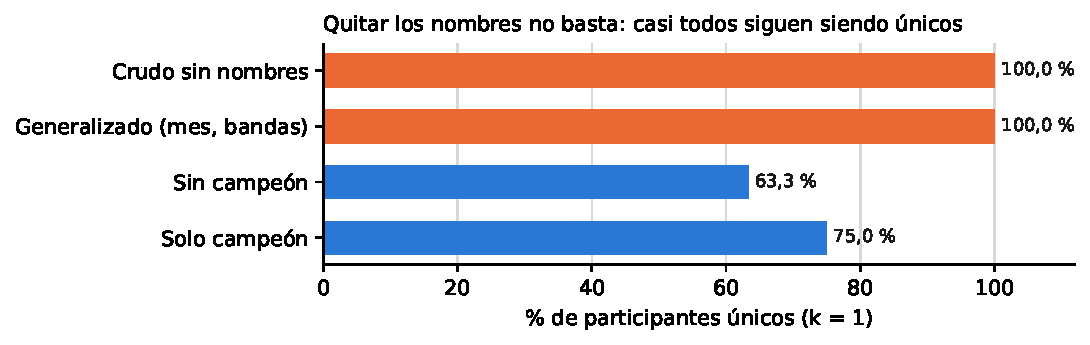
\includegraphics[width=\linewidth]{figuras/riesgo.pdf}
  \caption{Porcentaje de participantes únicos (\(k=1\)) en cada nivel de
  generalización.}
  \label{fig:riesgo}
\end{figure}

\noindent Tres lecturas:

\begin{enumerate}[leftmargin=1.6em,itemsep=.3em]
  \item \textbf{La generalización no movió nada:} \pctUnicosCrudo\,\% de únicos antes y
        \pctUnicosGen\,\% después. Pasar la fecha a mes y el nivel a bandas es
        correcto, pero no es lo que vuelve único a un participante: es el campeón.
        Con solo el campeón ya es único el \pctUnicosCampeon\,\%.
  \item \textbf{Quitar el campeón tampoco basta:} sin él sigue siendo único el
        \pctUnicosSinCampeon\,\%. Llegar a \(k \ge 2\) exigiría suprimir rol y
        parche también, y entonces no queda nada que analizar. Es el «punto de no
        retorno» de la clase: un conjunto anonimizado hasta ese grado ya no sirve.
  \item \textbf{A nivel partida, la composición es una huella:} las \compUnicas{} de
        \compTotal{} partidas 5v5 tienen una combinación de diez campeones única.
        Con la composición y el mes, alguien con acceso a una base grande de
        partidas (los sitios de estadísticas las recolectan) podría encontrar la
        partida y, con ella, los nombres.
\end{enumerate}

\noindent \textbf{Advertencia de tamaño:} \nPartidasCinco{} partidas son muy pocas, y
en un conjunto pequeño casi todo es único. Con la muestra real (se esperan
\(\sim\)200 partidas) los porcentajes bajarán, sobre todo el de «sin campeón». Por eso
el script recalcula esta tabla en cada corrida: se reporta de nuevo con los datos
propios, no se asume.

% ===========================================================================
\section{Decisiones para el proyecto}

La medición cambia lo que el proyecto va a publicar:

\begin{enumerate}[leftmargin=1.6em,itemsep=.35em]
  \item \textbf{Al repositorio público solo van tablas a nivel equipo.} La rúbrica del
        proyecto final pide un repositorio público para reproducir el análisis. Pero
        la sección~\ref{sec:riesgo} mostró que la tabla de participantes (campeón y
        rol de cada desconocido) es única fila por fila, así que \textbf{no se
        publica}. El script escribe aparte, en \texttt{salida/publico/}, lo único que
        el análisis de curvas y objetivos necesita: \texttt{partidas},
        \texttt{oro\_equipo} (oro por equipo y minuto) y \texttt{eventos\_equipo}
        (tipo, minuto y equipo de cada evento, sin campeones). Ahí ya no existe la
        composición de diez campeones que funcionaba como huella. El JSON crudo y las
        tablas por participante quedan en disco local, fuera del control de
        versiones.
  \item \textbf{Ningún \texttt{matchId} de partidas propias en las diapositivas.}
        Las diapositivas actuales muestran \texttt{EUW1\_6569580003}, que se puede
        porque es un ejemplo público de la documentación. Con partidas propias se
        usará el seudónimo.
  \item \textbf{Los campeones se conservan solo en local, y el riesgo se declara.} El
        análisis los usa, pero la composición completa de una partida no sale de la
        máquina. En las diapositivas se mostrará, a lo más, el campeón propio. El
        riesgo residual se dice en el reporte en lugar de esconderlo.
  \item \textbf{Las cifras se reportan agregadas.} El entregable final son
        frecuencias de arquetipos y curvas promedio, no tablas fila por fila de
        otros jugadores.
  \item \textbf{Equipo de cada evento por \texttt{killerId}, no por \texttt{teamId}.}
        Al construir \texttt{eventos\_equipo} se confirmó la trampa medida en el
        piloto: en \texttt{BUILDING\_KILL}, \texttt{teamId} nombra al equipo que
        \emph{perdió} la torre. Con la atribución correcta, las torres por equipo
        cuadran contra el conteo oficial del registro en 6 de 6 partidas.
\end{enumerate}

% ===========================================================================
\section{Conclusiones}

\begin{enumerate}[leftmargin=1.6em,itemsep=.4em]
  \item \textbf{Los identificadores directos son la parte fácil.} Se suprimen o
        seudonimizan con una regla por campo, y un barrido con control negativo
        demuestra que no quedó ninguno: \nFugas{} en la salida.
  \item \textbf{El peligro estaba en un campo con cara de técnico.} \texttt{matchId}
        no parece un dato personal, y sin embargo identifica a diez personas con
        una sola llamada a la API. Ningún campo se debe juzgar por su nombre.
  \item \textbf{Hash no es anonimización.} Un identificador con pocos valores
        posibles se revierte enumerando; por eso HMAC con llave, y llave efímera
        para que no exista tabla de correspondencia.
  \item \textbf{No hay modelo perfecto, y aquí se ve con números.} La
        generalización no bajó el \pctUnicosGen\,\% de participantes únicos, y
        alcanzar \(k\)-anonimato destruiría el análisis. La decisión honesta es
        conservar lo que el análisis necesita, publicar solo agregados y declarar el
        riesgo residual.
  \item \textbf{Para la siguiente etapa:} si el proyecto publica frecuencias por
        arquetipo, la privacidad diferencial (Dwork, 2006) sería el modelo
        adecuado para consultas. Pero con \(\sim\)100 derrotas el ruido necesario
        taparía la señal, así que por ahora se prefiere no publicar nada por debajo
        del nivel de agregado.
\end{enumerate}

% ===========================================================================
\section*{Referencias}
\addcontentsline{toc}{section}{Referencias}
\begin{itemize}[leftmargin=1.4em,itemsep=.3em,label={}]
  \item Dwork, C. (2006). Differential privacy. En \emph{Automata, Languages and
        Programming (ICALP 2006)}, LNCS 4052, 1--12. Springer.
  \item Pandurangan, V. (2014). \emph{On taxis and rainbows: Lessons from NYC's
        improperly anonymized taxi logs}. Medium.
  \item Reglamento (UE) 2016/679 del Parlamento Europeo y del Consejo (Reglamento
        General de Protección de Datos), art.~4.5 y considerando 26.
  \item Riot Games. \emph{Developer Portal — Policies}.
        \url{https://developer.riotgames.com/policies/general}
  \item Rocher, L., Hendrickx, J.~M., y de Montjoye, Y.-A. (2019). Estimating the
        success of re-identifications in incomplete datasets using generative
        models. \emph{Nature Communications}, 10, 3069.
        \url{https://doi.org/10.1038/s41467-019-10933-3}
  \item Sweeney, L. (2002). k-anonymity: A model for protecting privacy.
        \emph{International Journal of Uncertainty, Fuzziness and Knowledge-Based
        Systems}, 10(5), 557--570.
  \item Fuente de los datos: \texttt{MingweiSamuel/riotapi-schema}, ejemplos
        públicos de respuestas de \texttt{match-v5}.
\end{itemize}

\section*{Anexo: reproducir este reporte}
\addcontentsline{toc}{section}{Anexo: reproducir este reporte}
\begin{verbatim}
cd LoL_Anonimizacion
python scripts/anonimizar.py            # tablas/, figuras/, salida/*.csv
latexmk -pdf reporte_anonimizacion.tex
\end{verbatim}
\noindent El script sale con código 1 si el barrido encuentra cualquier identificador
en la salida, y falla si el control negativo no encuentra nada en el crudo.

\vspace{.5cm}
\noindent{\small\color{suave} Este proyecto no está avalado por Riot Games y no
refleja las opiniones de Riot Games ni de nadie involucrado oficialmente en la
producción o administración de League of Legends. League of Legends y Riot Games
son marcas registradas de Riot Games,~Inc.}

\end{document}
